% COMP8240 Project Update Presentation -- Min-K% Prob replication
% Compile: pdflatex slides.tex  (or upload this folder to Overleaf)
\documentclass[aspectratio=169,10pt]{beamer}
\usetheme[progressbar=frametitle,numbering=fraction]{metropolis}
\usepackage{booktabs}
\usepackage{tikz}
\usetikzlibrary{positioning,arrows.meta,shapes.geometric}
\usepackage{xcolor}

% Numbers come from the results files via scripts/make_figures.py; defaults show what is still pending.
\InputIfFileExists{numbers.tex}{}{}
% Fallbacks for numbers not produced yet (numbers.tex, generated by scripts/make_figures.py, wins).
\providecommand{\repPPL}{--}
\providecommand{\repZlib}{--}
\providecommand{\repLowercase}{--}
\providecommand{\repSmallerRef}{--}
\providecommand{\repMinK}{--}
\providecommand{\newBuilt}{(pending)}
\providecommand{\newN}{--}
\providecommand{\newNA}{--}
\providecommand{\newNB}{--}
\providecommand{\newNC}{--}
\providecommand{\newRejectedNon}{--}
\providecommand{\newCheckedNon}{--}
\providecommand{\blindWikiMIAtfidflr}{--}
\providecommand{\blindWikiMIAtfidflrnoyr}{--}
\providecommand{\blindarXivTectiontfidflr}{--}
\providecommand{\blindarXivLeaky}{--}
\providecommand{\blindMIMIRtfidflr}{--}
\providecommand{\newMinKSmall}{--}
\providecommand{\newMinKMid}{--}
\providecommand{\newMinKLarge}{--}
\providecommand{\newPPLLarge}{--}
\providecommand{\newZlibLarge}{--}


\definecolor{mqred}{HTML}{A6192E}
\definecolor{sblue}{HTML}{2A78D6}
\definecolor{sorange}{HTML}{EB6834}
\definecolor{saqua}{HTML}{1BAF7A}
\definecolor{ink2}{HTML}{52514E}
\setbeamercolor{frametitle}{bg=mqred!85!black}
\setbeamercolor{progress bar}{fg=sorange}
\newcommand{\muted}[1]{{\color{ink2}#1}}
\newcommand{\figorpending}[2]{\IfFileExists{#2}{\includegraphics[width=#1]{#2}}%
  {\fbox{\parbox[c][3.2cm][c]{#1}{\centering\muted{figure pending: \texttt{\detokenize{#2}}}}}}}

\title{Replicating Min-K\% Prob}
\subtitle{Project update: detecting pretraining data from large language models}
\author{Ashikur Rahman \quad\muted{48483818}}
\institute{COMP8240 Applications of Data Science, Macquarie University}
\date{9 October 2026 \quad\muted{github.com/Ashik-here/COMP8240-MinK-Replication}}

\begin{document}

\maketitle

% ---------------------------------------------------------------- RECAP
\begin{frame}{The question and the paper}
  \textbf{Can an outsider tell whether a text was in a model's training data?}\\
  \muted{Copyright, benchmark contamination, privacy: all need this ``membership inference''.}
  \vspace{0.6em}

  \begin{columns}[T]
    \begin{column}{0.56\textwidth}
      \textbf{Shi et al., ICLR 2024}
      \begin{itemize}\setlength\itemsep{2pt}
        \item ICLR: CORE \textbf{A*}, Google Scholar top-10 venue
        \item Code: \texttt{swj0419/detect-pretrain-code}\\ \muted{Apache-2.0, pinned at commit \texttt{a5048f9}}
        \item Data: WikiMIA on Hugging Face \muted{(MIT)}
      \end{itemize}
    \end{column}
    \begin{column}{0.42\textwidth}
      \textbf{Why this paper}
      \begin{itemize}\setlength\itemsep{2pt}
        \item runs on a free Colab T4
        \item $\sim$250 lines: I can explain all of it
        \item claim is \textbf{contested}\\ \muted{Duan et al.\ 2024; Das et al.\ 2024}
      \end{itemize}
    \end{column}
  \end{columns}
\end{frame}

\begin{frame}{The method: Min-K\% Prob}
  \begin{columns}[c]
    \begin{column}{0.55\textwidth}
      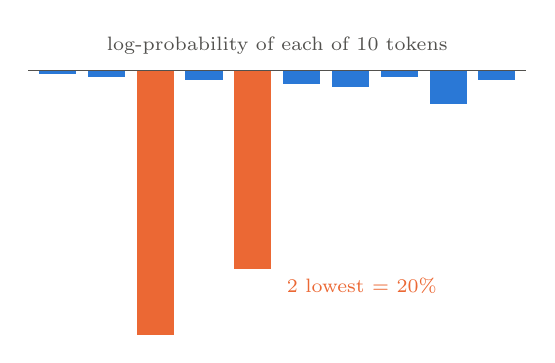
\begin{tikzpicture}[x=0.62cm,y=0.42cm]
        \foreach \i/\v in {1/0.1,2/0.2,3/8.0,4/0.3,5/6.0,6/0.4,7/0.5,8/0.2,9/1.0,10/0.3}{
          \pgfmathsetmacro{\c}{(\v>5)?1:0}
          \ifdim\c pt>0.5pt
            \fill[sorange] (\i-0.38,0) rectangle (\i+0.38,-\v);
          \else
            \fill[sblue] (\i-0.38,0) rectangle (\i+0.38,-\v);
          \fi
        }
        \draw[ink2] (0.4,0) -- (10.6,0);
        \node[ink2,font=\scriptsize,anchor=south] at (5.5,0.2) {log-probability of each of 10 tokens};
        \node[font=\scriptsize,anchor=west] at (5.5,-6.5) {\color{sorange}2 lowest = 20\%};
      \end{tikzpicture}
    \end{column}
    \begin{column}{0.43\textwidth}
      \begin{itemize}\setlength\itemsep{4pt}
        \item Average of \emph{all} tokens: $-1.7$
        \item Average of the \textbf{lowest 20\%}: $(-8.0-6.0)/2=\mathbf{-7.0}$
        \item Unseen text has a few very surprising words; training removes them
        \item Higher score $\Rightarrow$ predict \textbf{member}
        \item One forward pass, no reference model
      \end{itemize}
    \end{column}
  \end{columns}
\end{frame}

\begin{frame}{Original data: WikiMIA}
  \textbf{Labels come from dates, not from the model's (secret) training set}
  \begin{itemize}\setlength\itemsep{3pt}
    \item \textbf{Members}: Wikipedia event articles created \emph{before 2017}
    \item \textbf{Non-members}: event articles created \emph{after 1 Jan 2023}, after every model's cut-off
    \item Same passages cut to 32 / 64 / 128 / 256 words, balanced 50/50
  \end{itemize}
  \vspace{0.4em}
  \centering
  \begin{tabular}{lrrrr}
    \toprule
    Length (words) & 32 & 64 & 128 & 256 \\
    \midrule
    Passages & 776 & 542 & 250 & 82 \\
    \bottomrule
  \end{tabular}
  \vspace{0.5em}

  \muted{Metrics: AUC (chance = 0.5) and TPR at 5\% false-positive rate.}
\end{frame}

\begin{frame}{System architecture}
  \centering
  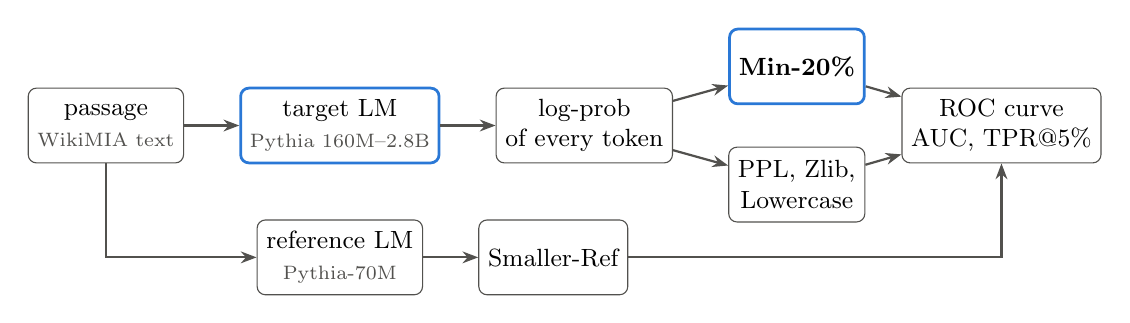
\begin{tikzpicture}[
      box/.style={draw=ink2,rounded corners=3pt,align=center,font=\small,minimum height=0.95cm,fill=white},
      hi/.style={box,draw=sblue,line width=1pt},
      arr/.style={-{Stealth[length=2mm]},ink2,thick}, node distance=0.55cm and 0.7cm]
    \node[box] (p) {passage\\\muted{\scriptsize WikiMIA text}};
    \node[hi,right=of p] (t) {target LM\\\muted{\scriptsize Pythia 160M--2.8B}};
    \node[box,right=of t] (lp) {log-prob\\of every token};
    \node[hi,right=of lp,yshift=0.75cm] (mk) {\textbf{Min-20\%}};
    \node[box,right=of lp,yshift=-0.75cm] (bl) {PPL, Zlib,\\Lowercase};
    \node[box,below=0.7cm of t] (r) {reference LM\\\muted{\scriptsize Pythia-70M}};
    \node[box,right=of r,xshift=0.0cm] (sr) {Smaller-Ref};
    \node[box,right=2.9cm of lp] (roc) {ROC curve\\AUC, TPR@5\%};
    \draw[arr] (p) -- (t); \draw[arr] (t) -- (lp);
    \draw[arr] (lp) -- (mk); \draw[arr] (lp) -- (bl);
    \draw[arr] (p) |- (r); \draw[arr] (r) -- (sr);
    \draw[arr] (mk) -- (roc); \draw[arr] (bl) -- (roc); \draw[arr] (sr) -| (roc);
  \end{tikzpicture}
  \vspace{0.6em}

  \raggedright
  \texttt{run.py} scores each passage $\rightarrow$ \texttt{eval.py} writes \texttt{auc.txt} + ROC plot.\\
  \muted{I import the original functions unmodified and call them from a notebook, so per-passage
  scores are kept (the original script discards them).}
\end{frame}

% ---------------------------------------------------------------- UPDATE
\begin{frame}{Replication on original data: status}
  \begin{columns}[c]
    \begin{column}{0.40\textwidth}
      \small
      \textbf{Pythia-2.8B, mean of 4 lengths}\\[3pt]
      \begin{tabular}{lcc}
        \toprule
        Method & Mine & Paper \\
        \midrule
        PPL         & \repPPL        & 0.61 \\
        Zlib        & \repZlib       & 0.65 \\
        Lowercase   & \repLowercase  & 0.59 \\
        Smaller Ref & \repSmallerRef & 0.60 \\
        \textbf{Min-20\%} & \textbf{\repMinK} & \textbf{0.67} \\
        \bottomrule
      \end{tabular}\\[5pt]
      \textbf{All five within 0.02 of the paper.}\\[1pt]
      size \repMinSmall$\,\rightarrow\,$\repMinLarge,\; length \repMinLenShort$\,\rightarrow\,$\repMinLenLong\\[1pt]
      \muted{Min-K\% leads Zlib by $<$0.01: inside the CIs.}\\[3pt]
      \muted{\scriptsize Colab T4, original code at \texttt{a5048f9}, transformers 5.18, fp16.}
    \end{column}
    \begin{column}{0.59\textwidth}
      \figorpending{\linewidth}{figures/auc_vs_size.pdf}\\[2pt]
      \muted{\footnotesize Scope: the paper's 20B--66B models exceed a free T4, so its size claim is
      tested across five Pythia sizes instead.}
    \end{column}
  \end{columns}
\end{frame}

\begin{frame}{What replication needed: five traps in the original repo}
  \begin{enumerate}\setlength\itemsep{3pt}
    \item No \texttt{requirements.txt} $\Rightarrow$ I pin and record versions myself
    \item Imports \texttt{openai} always; GPT-3 rows use \texttt{text-davinci-003}, \textbf{retired}
          \muted{$\Rightarrow$ those rows can never be reproduced}
    \item Score stored negated, then negated again in \texttt{eval.py}
          \muted{$\Rightarrow$ a re-implementation can silently flip the ROC}
    \item A committed \texttt{out/} folder holds the \emph{authors'} LLaMA-13B results
          \muted{$\Rightarrow$ easy to read theirs instead of yours}
    \item \texttt{auc.txt} says ``TPR@0.1\%FPR'' but the code computes TPR@\textbf{5\%}
  \end{enumerate}
  \vspace{0.3em}
  \muted{Also: Table 1 does not say which length it reports, so I report all four plus the mean.
  Independent 30-line re-implementation matches the repo to 3 decimals.}
\end{frame}

\begin{frame}{New data 1: existing datasets the paper did not use}
  \begin{columns}[T]
    \begin{column}{0.5\textwidth}
      \textbf{arXivTection} \muted{(DE-COP, ICML 2024)} \hfill\textcolor{saqua}{\textbf{done}}
      \begin{itemize}\setlength\itemsep{2pt}
        \item 50 arXiv papers, \textbf{1,549} passages
        \item label: published before 2022 vs.\ in 2023
        \item shipped as multiple choice $\Rightarrow$ adapter keeps the verbatim option
        \item \muted{caveat: labels suit 2022+ models, not Pythia}
      \end{itemize}
    \end{column}
    \begin{column}{0.48\textwidth}
      \textbf{MIMIR} \muted{(COLM 2024)} \hfill\textcolor{saqua}{\textbf{obtained}}
      \begin{itemize}\setlength\itemsep{2pt}
        \item Pile \emph{train} vs.\ \emph{test}: same time, same sources
        \item built for Pythia: my primary target
        \item \textbf{gated} since my proposal $\Rightarrow$ access granted today;
              Wikipedia split, 1,000 + 1,000 passages
        \item \muted{kept local: gated data is not redistributed}
      \end{itemize}
      \vspace{0.3em}
      \textbf{BookTection}: public, same adapter \hfill\muted{next}
    \end{column}
  \end{columns}
\end{frame}

\begin{frame}{New data 2: WikiMIA-2026, built with the paper's own recipe}
  \begin{columns}[T]
    \begin{column}{0.56\textwidth}
      \small
      \textbf{Pipeline} \muted{(\texttt{scripts/build\_wikimia2026.py})}
      \begin{enumerate}\setlength\itemsep{1pt}
        \item MediaWiki API: event categories of 2026 vs.\ 2012--15
        \item creation date = first revision; keep $\geq$ 1 Jan 2026 / $<$ 2017
        \item drop ``List of\ldots'', ``Timeline of\ldots''; regex clean
        \item cut to 32/64/128/256 words, balance 50/50
        \item JSONL in the original schema $\Rightarrow$ \texttt{run.py} unmodified
      \end{enumerate}
      \textbf{Change from WikiMIA:} \emph{same} 16 topic types on both sides.\\[6pt]
      \textbf{First attack result} \muted{(original code, Pythia-2.8B)}:\\
      Min-K\% \textbf{\newMinKLarge} \muted{(WikiMIA \repMinK)}, PPL \newPPLLarge, Zlib \newZlibLarge;
      size \newMinKSmall\,$\rightarrow$\,\newMinKMid\,$\rightarrow$\,\newMinKLarge\\
      $\Rightarrow$ \textbf{the claim transfers to fresh data}
    \end{column}
    \begin{column}{0.42\textwidth}
      \small
      \textbf{Built \newBuilt}\\[2pt]
      \begin{tabular}{lr}
        \toprule
        Length & Passages \\
        \midrule
        32 & \newN \\ 64 & \newNA \\ 128 & \newNB \\ 256 & \newNC \\
        \bottomrule
      \end{tabular}\\[3pt]
      \muted{\scriptsize \newRejectedNon\ of \newCheckedNon\ ``2026'' pages were created \emph{before}
      2026 and rejected. Each passage keeps page id, revision id, creation time.}\\[6pt]
      \textbf{Annotation:} membership labels come \emph{automatically} from creation dates.\\
      \muted{Human + LLM-judge labels: planned for the recency audit (ND-2).}
    \end{column}
  \end{columns}
\end{frame}

\begin{frame}{Progress: does the benchmark leak its own labels?}
  \begin{columns}[c]
    \begin{column}{0.64\textwidth}
      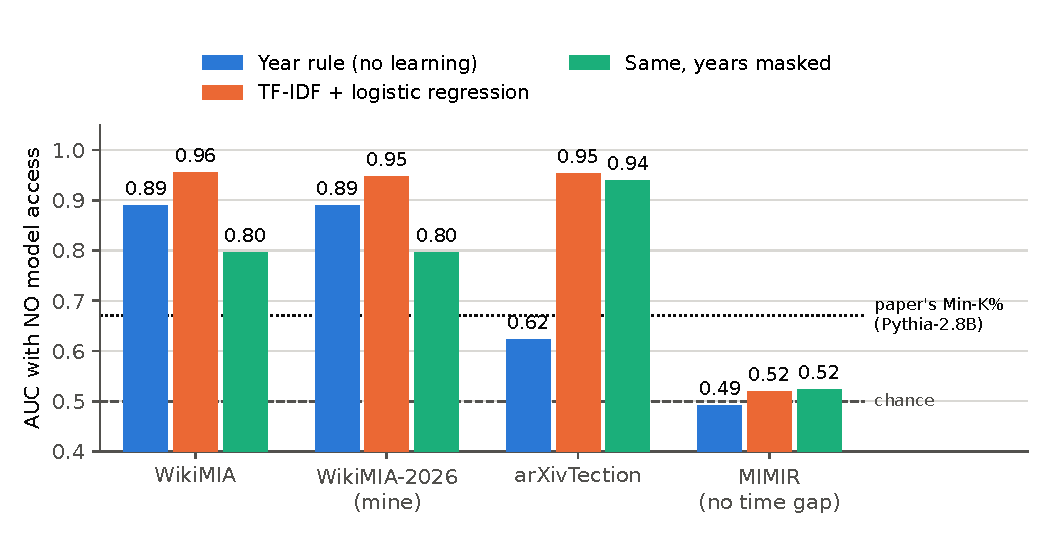
\includegraphics[width=\linewidth]{figures/blind_audit.pdf}\\
      \muted{\scriptsize WikiMIA bars: mean over the 4 lengths; 5-fold CV inside a pipeline
      (arXivTection: folds grouped by paper).}
    \end{column}
    \begin{column}{0.35\textwidth}
      \footnotesize
      AUC of a classifier that \textbf{never sees the model}:
      \begin{itemize}\setlength\itemsep{1pt}
        \item WikiMIA \textbf{\blindWikiMIAtfidflr} \muted{(Min-K\%: 0.67)}
        \item years masked \blindWikiMIAtfidflrnoyr\ \muted{(``will be'' vs.\ ``was'')}
        \item my WikiMIA-2026 \textbf{\blindWikiMIANewtfidflr} \muted{(topics matched)}
        \item arXivTection \blindarXivTectiontfidflr\ \muted{(\blindarXivLeaky\ if folds leak papers)}
        \item \textbf{control} MIMIR \textbf{\blindMIMIRtfidflr} $\approx$ chance
      \end{itemize}
      \vspace{2pt}
      $\Rightarrow$ the leak is \textbf{time}, not memorisation.
    \end{column}
  \end{columns}
\end{frame}

\begin{frame}{Next steps}
  \begin{enumerate}\setlength\itemsep{4pt}
    \item \textbf{Min-K\% on MIMIR}, where the blind baseline is at chance: does the attack still beat 0.5?
    \item \textbf{ND-2: a shift-controlled split}: members and non-members from the same time window;
          blind AUC must be $\approx 0.5$ \emph{before} any attack is trusted
    \item Which passages does Min-K\% get right: the same ones the blind classifier finds easy?
    \item LLM-as-judge recency check \muted{(both A/B orders)} + 200 human labels, Cohen's / Fleiss' $\kappa$;
          final report in \LaTeX{} with the GitHub repo
  \end{enumerate}
  \vspace{0.4em}
  \centering
  \textbf{So far:} the method reproduces on old \emph{and} new data;\\
  the open question is whether it detects \emph{memorisation} or \emph{time}.\\[0.7em]
  \fcolorbox{sblue}{sblue!8}{\parbox{0.86\textwidth}{\centering\small
    \textbf{All code, data, results and run logs:}\quad
    \texttt{\href{https://github.com/Ashik-here/COMP8240-MinK-Replication}{github.com/Ashik-here/COMP8240-MinK-Replication}}}}
\end{frame}

\end{document}
